\documentclass[a4paper]{article}
\usepackage{graphicx, caption}
\usepackage{setspace}
\usepackage{url}
\usepackage{underscore}
\usepackage{caption}
\usepackage{subcaption}
\usepackage{siunitx}
\usepackage{amsmath}
\usepackage[a4paper,margin=1in,footskip=0.25in]{geometry}
\usepackage{indentfirst}

\setlength{\parindent}{1.5cm}
\setlength{\parskip}{0.5em}

%opening
\title{ 
	\begin{center}
		\textbf{Enhancing Small Object Detection with Lite FPN SSD: A Minimal Parameter Addition for Significant Improvements}
	\end{center}
}

\author{PhD.Duong Viet Hang, Nguyen Dang Duc Manh\\ University of Information Technology (UIT) \\ \texttt{hangdv@uit.edu.vn, 22520847@gm.uit.edu.vn}}

\begin{document}
	
	\maketitle
	
	\begin{abstract}
	Small object detection is a challenging task in computer vision, as detecting and accurately localizing these objects often proves difficult for many object detection models. In this paper, we propose a novel approach called Lite FPN SSD that addresses this issue by making a minimal addition of only 2 million parameters while achieving remarkable improvements in detecting small objects. Through experimentation on VOC, and COCO datasets, we demonstrate that Lite FPN SSD achieves impressive results. Specifically, our model achieves a mean average precision (mAP) of 78.36\% on the VOC dataset and on the COCO dataset, Lite FPN SSD achieves a competitive mAP of 46.27\% outperforming some existing improved models from other author. Lite FPN SSD builds upon the popular Feature Pyramid Network (FPN) and Single Shot MultiBox Detector (SSD) architectures, leveraging their strengths in feature extraction and efficient object detection. By effectively capturing and utilizing multi-scale features, our approach enables enhanced localization and recognition of small objects. Furthermore, Lite FPN SSD maintains competitive performance on larger objects, making it a versatile solution for diverse object detection tasks. Its lightweight nature, with a minimal increase in parameters, ensures high efficiency for real-time applications.

	
	\end{abstract}
	
	\section{Introduction}	
		
	Object detection is a fundamental task in computer vision that involves identifying and localizing objects within an image. Over the years, several approaches have been developed to tackle this problem, ranging from two-stage detectors to more recent one-stage detectors.
	
	\begin{center}
		\begin{minipage}{1.0\linewidth}
			\centering
			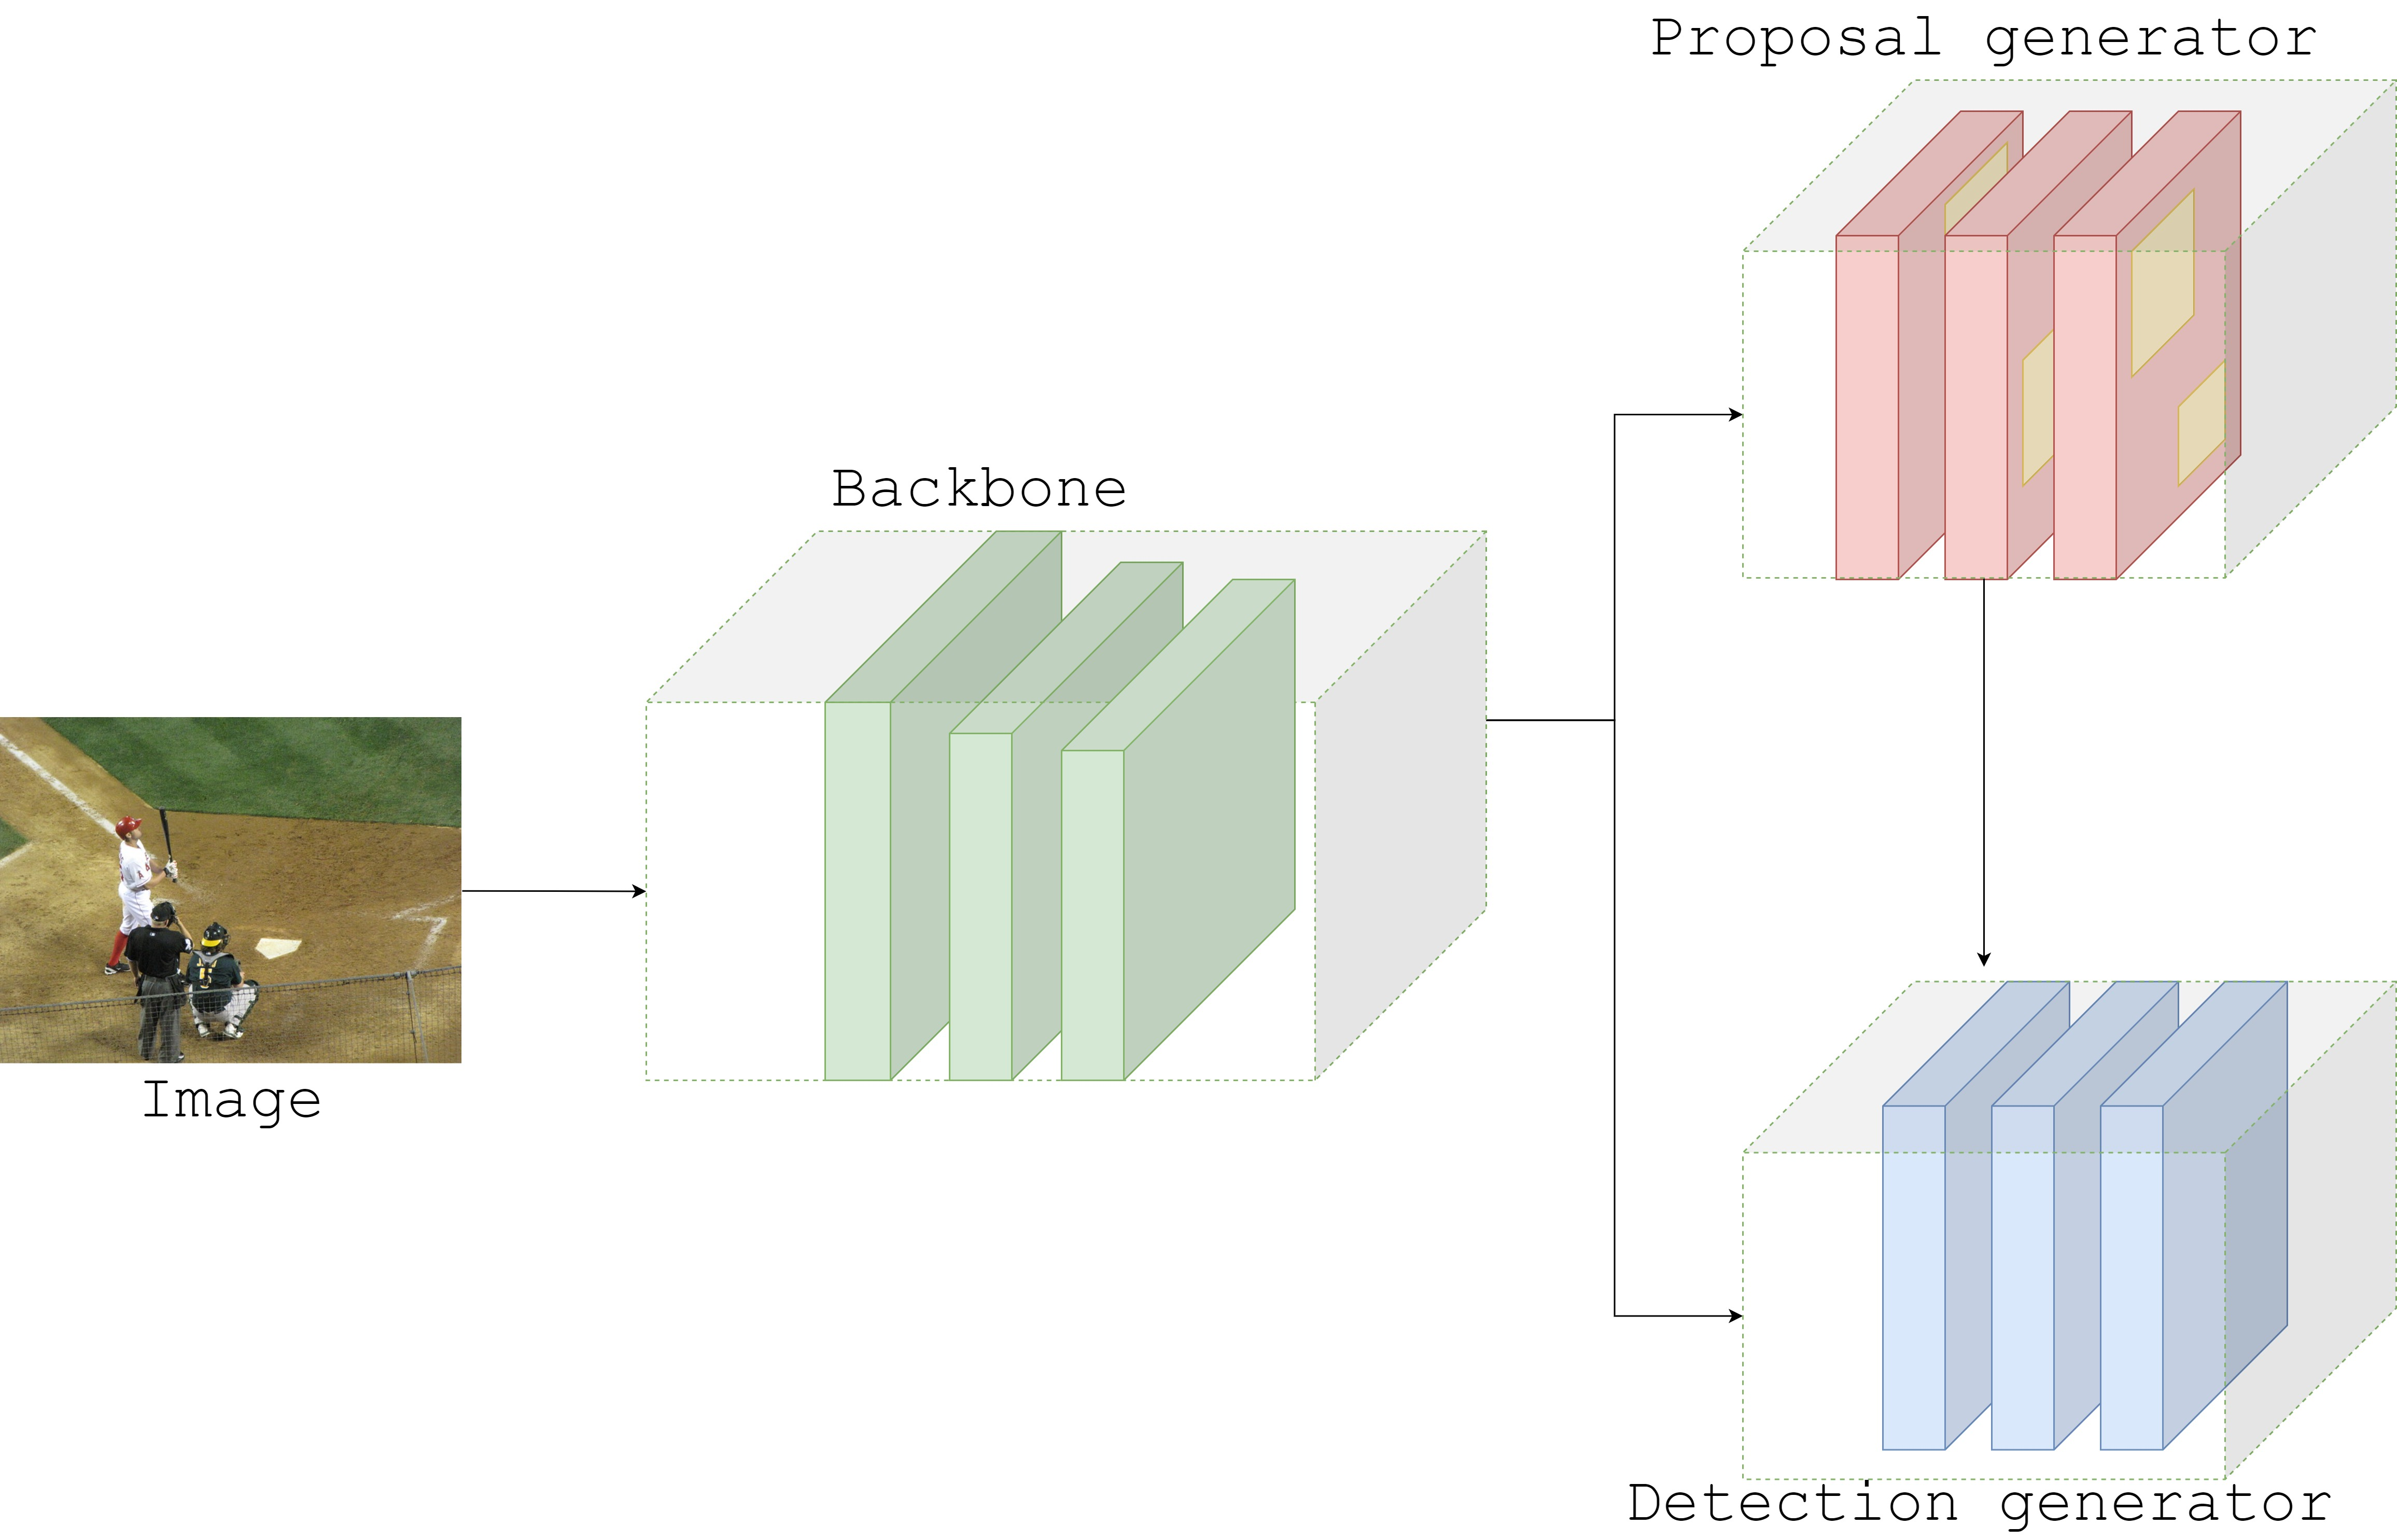
\includegraphics[width=0.7\linewidth]{../../project_WPD/fig/Two_stage}
			\captionsetup{labelformat=empty} % Không hiển thị số thứ tự caption
			\captionsetup{labelformat=empty} % Không hiển thị số thứ tự caption
			\captionof{figure}{b.) Two-stage detector}
			
		\end{minipage}
		
		\vspace{1cm}
		
		\begin{minipage}{1.0\linewidth}
			\centering
			\includegraphics[width=0.7\linewidth]{../../project_WPD/fig/One_stage}
			\captionsetup{labelformat=empty} % Không hiển thị số thứ tự caption
			\captionof{figure}{b.) One-stage detector}
			
		\end{minipage}
		\captionof{figure}{Two type of detection model}
		\label{detection}
	\end{center}
	
	One-stage detectors are a class of object detection models that aim to directly predict object bounding boxes and class labels in a single pass through the network. These models eliminate the need for a separate region proposal stage (see Fig~\ref{detection}), making them faster and simpler compared to two-stage detectors. One-stage detectors have gained significant popularity in recent years due to their efficiency and competitive performance. Several notable one-stage detectors have been proposed such as RetinaNet \cite{focalloss}, You Only Look Once (YOLO) and variations \cite{yolov1, yolov2, yolov3}, Single Shot MultiBox Detectors (SSD) \cite{ssd}, each with its unique characteristics and contributions. Among these models, SSD stands out as a widely adopted and influential approach in the field of object detection.


	The Single Shot MultiBox Detector (SSD) is a real-time object detection framework that combines high detection accuracy with efficient inference speed. It operates by dividing the input image into a grid of predefined anchor boxes at multiple scales and aspect ratios. For each anchor box, SSD predicts the object class probabilities and adjusts the bounding box offsets to accurately localize objects.

	SSD offers several advantages in object detection. Firstly, it leverages multiple feature maps at different scales, enabling it to capture objects of varying sizes effectively. This multi-scale feature fusion allows SSD to handle both small and large objects robustly. Secondly, SSD is a single-shot detector, meaning it performs object detection in a single pass through the network, making it highly efficient for real-time applications. Moreover, SSD achieves competitive accuracy on various object detection benchmarks.

	However, despite its strengths, SSD also has certain limitations, particularly in detecting small objects. The predefined anchor boxes may not adequately cover the variations in small object sizes, leading to challenges in accurate localization. Additionally, smaller objects may lack sufficient spatial context within a single feature map, affecting detection performance.

	To address these limitations and further improve the performance of SSD, researchers have proposed various enhancements and modifications. A few works that can be highlighted include using Fyture Pyramid Network \cite{fpn} on SSD \cite{fpnssd}, apply Enhanced Feature Map Block \cite{ssdemb}, using Feature Fusion Module \cite{fssd} and using Deconvolution Module \cite{dssd, mdssd}. One of the notable strengths of these models is their ability to achieve substantial improvements in mAP on benchmark datasets such as VOC and COCO, indicating their superior performance in object detection tasks. However, one notable drawback of these models is the substantial increase in the number of parameters Fig~\ref{tt}, which can lead to increased computational complexity, memory requirements and challenges in deploying them on resource-constrained devices or in real-time applications.
	
	\begin{center}
		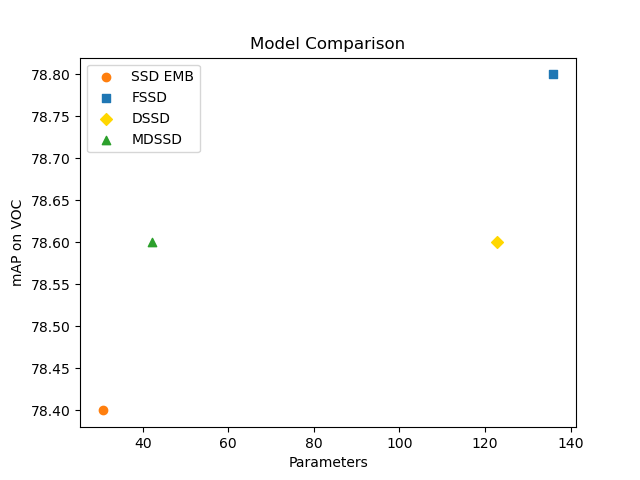
\includegraphics[width=0.7\linewidth]{../fig/param_mAP_VOC}
		\captionof{figure}{Numbers of paremeters and mAP on VOC 2007 test}
		\label{tt}
	\end{center}
	
	In this paper, we propose Lite FPN SSD, an innovative model that combines the strengths of SSD (Single Shot MultiBox Detector) and FPN (Feature Pyramid Network) \cite{fpn}. Our Lite FPN SSD model offers a significant advantage by introducing a mere 2 million additional parameters, while achieving exceptional mAP scores of 78.36 on the VOC dataset and 46.27 on the COCO dataset. This remarkable performance highlights the effectiveness of our model in striking a balance between parameter efficiency and superior accuracy.
	
	\section{Related works}
	
	\textbf{Single Shot Multibox Detector:} SSD is a popular object detection model known for its real-time inference capability \cite{ssd}. It combines a base network with convolutional layers to predict object class labels and bounding box coordinates at multiple scales and aspect ratios. SSD excels in achieving a balance between accuracy and speed, making it suitable for real-time applications. However, a weakness of SSD lies in its performance on detecting small objects. The reliance on fixed-size anchor boxes can hinder accurate localization and detection of small objects, resulting in lower precision and recall.
	
	\textbf{SSD-EMB:} an improved version of SSD (Single-Shot MultiBox Detector) that incorporates enhanced feature map blocks \cite{ssdemb}. SSD-EMB includes an attention stream and a feature map concatenation stream. The attention stream focuses on object regions using channel averaging and normalization, while the feature map concatenation stream adds semantic information without sacrificing detection speed. By combining these streams, SSD-EMB achieves enhanced feature maps for improved small object detection. Experimental results demonstrate the model's high accuracy in detecting small objects.
	
	\textbf{Feature Fusion Single Shot Multibox Detector:} FSSD is an enhanced version of SSD that incorporates a lightweight feature fusion module \cite{fssd}. By concatenating features from different layers with varying scales and generating a new feature pyramid, FSSD significantly improves detection performance while only slightly impacting speed. The feature fusion module enables FSSD to capture richer information from the input image, leading to enhanced accuracy in object detection. Overall, FSSD offers a powerful and efficient solution for accurate and fast object detection tasks.
	
	\textbf{Multi-Scale Deconvolutional Single Shot Detector:} MDSSD is a specialized model for small object detection \cite{mdssd}. It addresses this challenge by upsampling multiple high-level feature maps at different scales simultaneously, increasing spatial resolution. The Fusion Block integrates low-level feature maps through skip connections, producing fusion feature maps with strong representation power for small instances. Unlike the top-most layer, these fusion feature maps preserve semantic information and fine details crucial for small object detection. MDSSD effectively combines multi-scale deconvolution and fusion techniques to improve small object detection performance.
	
	\textbf{The Feature Pyramid Network:} FPN takes advantage of the inherent multi-scale and pyramidal structure of deep convolutional networks \cite{fpn}. It constructs feature pyramids with minimal additional cost and uses a top-down architecture with lateral connections. FPN serves as a highly effective feature extractor, improving performance in object detection, segmentation, and classification tasks. It achieves this by capturing fine-grained details and high-level semantic information at all scales, making it a valuable tool in computer vision applications.
	
	\textbf{Warm-up Learning Rate:} is a technique that gradually increases the learning rate from a small value to a desired level during model training \cite{warmup}. It improves stability and convergence speed by allowing the model to explore the data structure initially and avoid local minima. This approach is particularly useful for training large or challenging models, ensuring better performance and preventing oscillations during optimization.
	
	\section{Method}
	\subsection{SSD architecture}
	The SSD (Single Shot Multibox Detector) architecture is composed of a backbone network, multiscale feature maps, and detection layers. The backbone network, such as VGG16, serves as the foundation for feature extraction from the input image. It extracts features at different levels, allowing the model to capture objects of various sizes, see Fig~\ref{ssdarchitecture}.
	
	\begin{center}
		\includegraphics[width=1.0\linewidth]{../fig/SSD300}
		\captionof{figure}{SSD architecture}
		\label{ssdarchitecture}
	\end{center}
	
	The multiscale feature maps are obtained from different layers of the backbone network. These feature maps provide a hierarchical representation of the image, with earlier layers capturing fine-grained details and smaller objects, while deeper layers focus on larger objects with reduced spatial resolution. Detection layers are added on top of the feature maps to perform the final object detection tasks. These layers consist of convolutional operations that handle the classification of objects into predefined classes and the regression of bounding box coordinates.
	
	\subsection{FPN architecture}
	
	We have integrated FPN (Feature Pyramid Network) into the architecture of SSD (Single Shot Multibox Detector) to create a new framework called Lite FPN-SSD. This lightweight architecture aims to leverage the strengths of both models while maintaining a compact design. By combining the efficiency of SSD in detecting general objects and the advantage of FPN in detecting small objects, Lite FPN-SSD aims to provide improved performance across a wide range of object scales. Below is an illustration of the Lite FPN-SSD architecture:
	
	\begin{center}
		\includegraphics[width=1.1\linewidth]{../fig/FPNSSD300}
		\captionof{figure}{Lite FPNSSD architecture}
		\label{LiteFPNSSDarchitecture}
	\end{center}
	
	
	\subsection{FPN Module}
	In the proposed architecture, we have incorporated a critical module called the FPN Module. To assess the performance of FPN-SSD, we conducted experiments using three different modules, each corresponding to a model with varying parameter counts.
	
	The first module, SSD-Base, has a parameter count of 27.6 million. It represents a specific configuration of the SSD model and serves as the starting point for evaluating the subsequent modules, see Fig.
	
	\begin{center}
		
\includegraphics[width=1.1\linewidth]{../fig/Module_a}
		\captionof{figure}{Moudle a}
		\label{modulea}
	\end{center}
	
	The second module, SSD-Lite, has a parameter count of 28.3 million. It is designed to be a lightweight variant of the SSD model, offering a balance between model complexity and resource efficiency, see Fig.
	
	\begin{center}
		\includegraphics[width=0.95\linewidth]{../fig/Module_b}
		\captionof{figure}{Moudle b}
		\label{moduleb}
	\end{center}
	
	The third module, FPN-SSD, has a parameter count of 29.7 million. It incorporates the Feature Pyramid Network (FPN) module into the SSD model, aiming to enhance object detection capabilities, particularly for small objects, see Fig.
	
	\begin{center}
		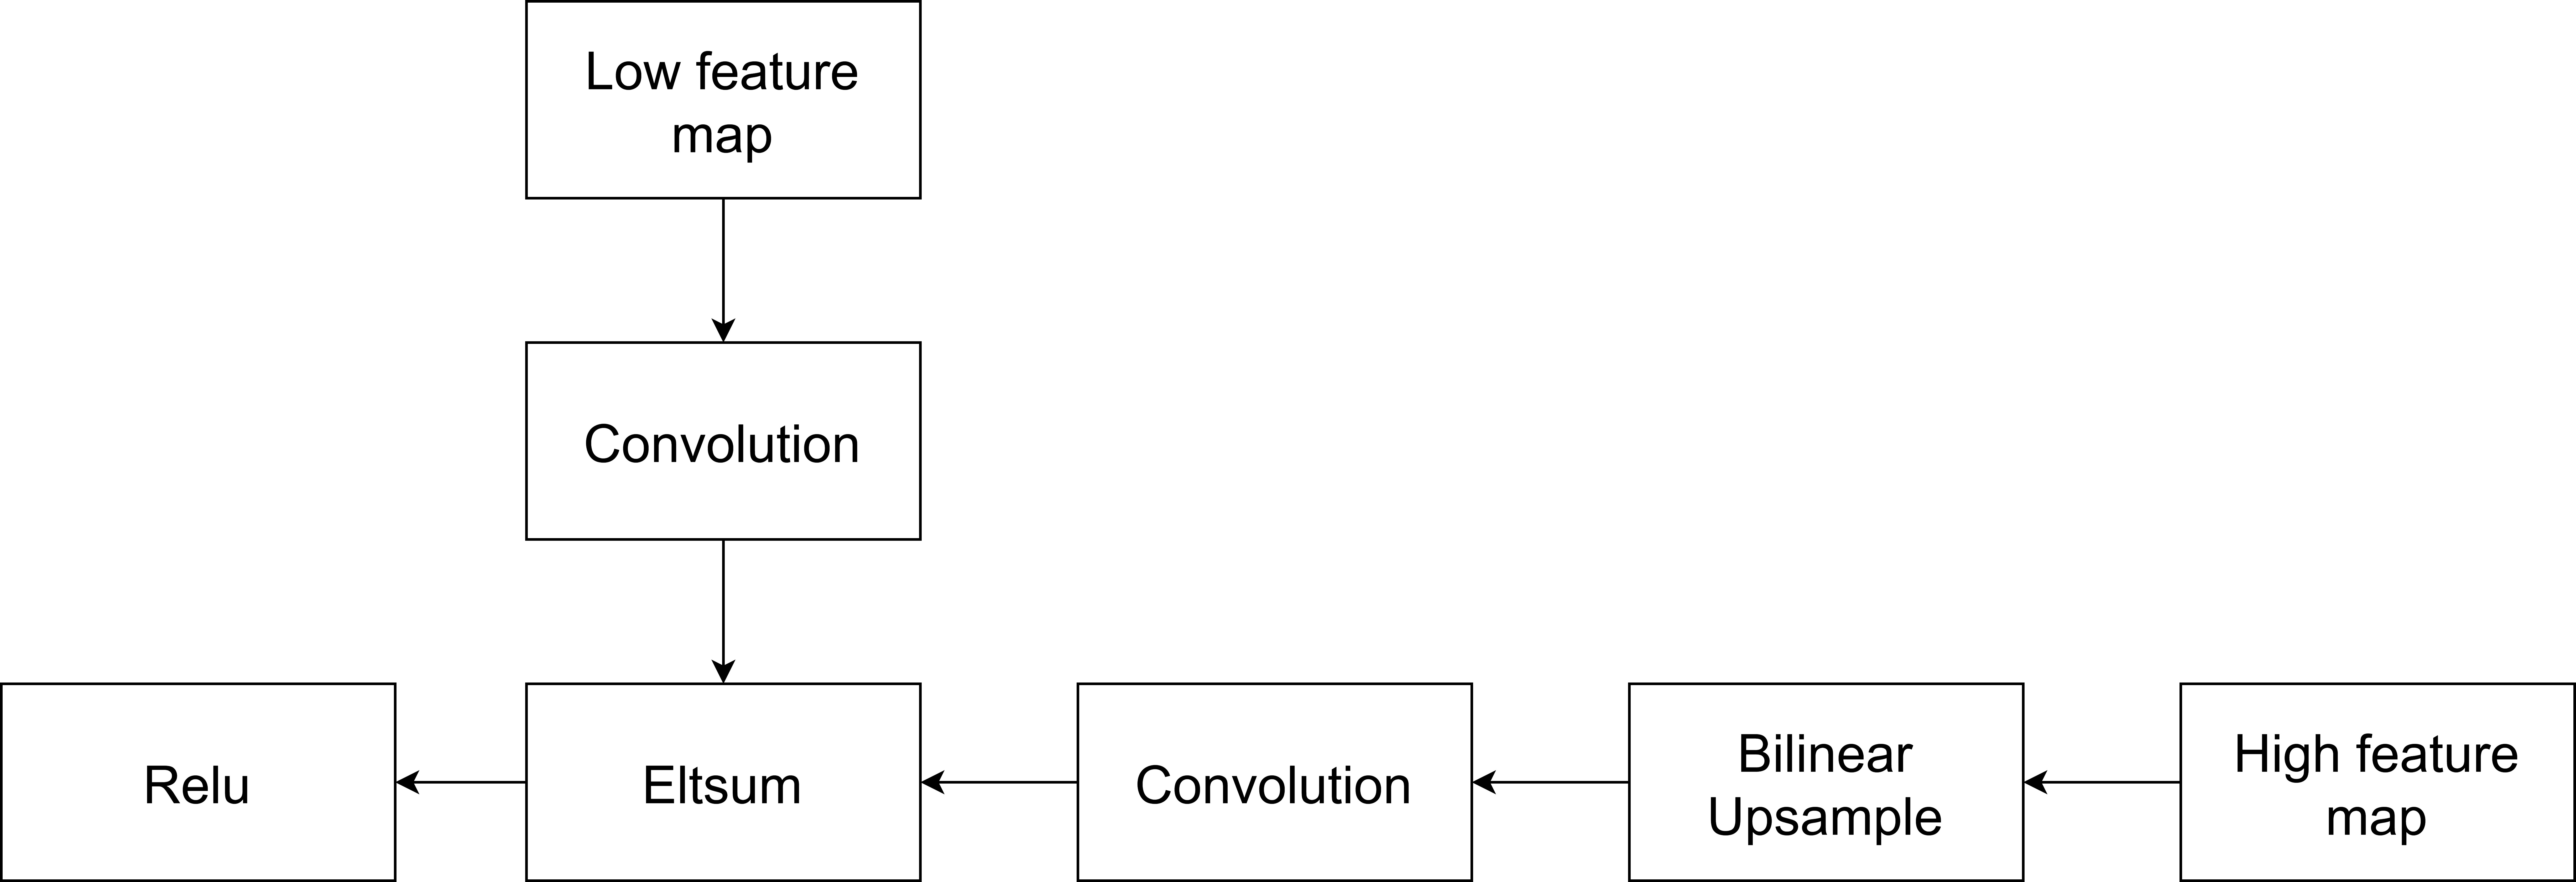
\includegraphics[width=0.95\linewidth]{../fig/Module_c}
		\captionof{figure}{Moudle c}
		\label{modulec}
	\end{center}
	
	It is important to note that the parameter count alone does not necessarily determine the performance or effectiveness of a module. The actual performance of each module in terms of object detection accuracy and efficiency should be evaluated through comprehensive experiments and analysis.
	
	The selection of a module depends on the specific requirements, constraints, and trade-offs of the application. It is essential to consider factors such as computational resources, real-time processing needs, and the desired level of object detection performance when choosing the most suitable module for a particular use case.
		
		
	\section{Experiment}
	
	\subsection{Training}
	
	\subsubsection{Training Objective}
	
	Before delving into the loss function, let us establish a set of notations for clarity in presentation:

	\begin{itemize}
		\item $x_{ij}^k$: an indicator function, where $x_{ij}^p \in \lbrace 0, 1 \rbrace$. $x_{ij}^k = 1$ indicates that the default box $i$ is matched with the ground truth box $j$ for object class $k$, while $x_{ij}^k = 0$ represents the opposite case.
		\item $\lbrace cx, cy, w, h \rbrace$: respectively denote the center coordinates along the horizontal axis ($cx$) and vertical axis ($cy$), as well as the width ($w$) and height ($h$) of a default box.
		\item $p$: the predicted offset, represented as $\lbrace \nabla{cx}, \nabla{cy}, \nabla{w}, \nabla{h} \rbrace$, which is the displacement estimated by the model.
		\item $g$: the ground truth, which is the expected object prediction, expressed as $\lbrace cx, cy, w, h \rbrace$.
		\item $d$: the default box, expressed as $\lbrace cx, cy, w, h \rbrace$.
		\item $c$: the probability vector for each class, denoted as $\lbrace prob_1, prob_2, \ldots, prob_n \rbrace$.
		\item $Pos$: the set of matched default boxes.
		\item $Neg$: the set of unmatched default boxes.
	\end{itemize}
	
	
We aim to minimize the loss function given by:

\begin{align}
	\mathcal{L}(p, d, g) &= \frac{1}{N}(\mathcal{L}_{conf}(c) + \alpha \mathcal{L}_{loc}(l, g)) 
\end{align} 

where $N$ represents the number of matched default boxes. If $N=0$, we assign a loss value of $0$. Here, $\alpha$ is a tunable parameter. The overall loss function $\mathcal{L}$ is the sum of two smaller component losses, $\mathcal{L}_{conf}$ and $\mathcal{L}_{loc}$.

Loss function for localization:

\begin{align}
	\mathcal{L}_{loc}(p, g) &= \sum_{i \in Pos}^{N} \sum_{m \in \lbrace cx, cy, w, h\rbrace} x_{ij}^{k} smooth_{L1}(p_i^m - \hat{g}_j^m)
\end{align} 

It is important to note that the notation $\hat{g}$ is distinct from $g$. Here, $g$ represents the original coordinates, while $\hat{g}$ denotes the normalized coordinates using the following formulas:

\begin{align}
	\hat{g}_j^{cx} &= \frac{(g_j^{cx} - d_i^{cx})}{d_i^w} \\ 
	\hat{g}_j^{cy} &= \frac{(g_j^{cx} - d_i^{cy})}{d_i^h} \\
	\hat{g}_j^w    &= \log(\frac{g_j^w}{d_i^w}) \\
	\hat{g}_j^h    &= \log(\frac{g_j^h}{d_i^h})
\end{align}

Loss function for confidence (probability):

\begin{align}
	\mathcal{L}_{conf}(c) = - \sum_{i \in Pos}^N x_{i, j}^k \log(\hat{c}_i^k) - \sum_{i \in Neg} log(\hat{c}_i^0), ~ where ~ \hat{c}_i^k = \frac{\exp(c_i^k)}{\sum_{k} \exp(c_i^k)}
\end{align}


By minimizing these component losses, we can effectively optimize the overall loss function, facilitating accurate object localization and confidence estimation.
 	
\subsubsection{Data augmetation}

In order to enhance the training process and improve the model's ability to detect objects, several data augmentation techniques are employed.

\begin{itemize}
	\item Random Adjustments: The image undergoes random adjustments to brightness, contrast, saturation, and hue. Each adjustment has a 50\% chance of being applied, and the order of adjustments is randomized.

	\item Zoom Out: With a 50\% probability, a zoom out operation is performed on the image. This operation helps the model learn to detect small objects. The zoomed out image is resized to be between 1 and 4 times larger than the original. The surrounding space is filled with the mean values of the ImageNet data.

	\item Random Crop: The image is randomly cropped, simulating a zoom in operation. This aids in learning to detect large or partially visible objects. The crop dimensions are randomly chosen between 0.3 and 1 times the original dimensions, ensuring variability in the crops. The aspect ratio of the crop is between 0.5 and 2. To maintain diversity, each crop retains at least one bounding box with a Jaccard overlap of 0, 0.1, 0.3, 0.5, 0.7, or 0.9, randomly selected. Bounding boxes whose centers are no longer within the cropped image are discarded. There is also a chance that the image remains uncropped.

	\item Horizontal Flip: The image is horizontally flipped with a 50\% chance. This augmentation technique increases the variability of the training data.

	\item Resize: The image is resized to a fixed size of 300x300 pixels. This specific size is a requirement of the SSD300 model.

	\item Convert to Fractional Coordinates: All bounding boxes are converted from absolute coordinates to fractional boundary coordinates. This conversion ensures consistency throughout the model, as all boundary and center-size coordinates are represented in fractional form.

	\item Image Normalization: The image is normalized using the mean and standard deviation values of the ImageNet data used to pretrain the VGG base. This normalization step aligns the image data with the pretrained model's expectations.
\end{itemize}

\subsubsection{General Training Parameters}

	In this section, we present the fixed set of parameters that remain constant throughout all experiments. These parameters provide a consistent framework for training and serve as the baseline configuration. The specific details of these shared parameters will be documented in the accompanying table below. This allows for a clear and concise overview of the parameters that are consistent across all datasets.
	
	
\begin{center}
	\includegraphics[width=0.7\linewidth]{"../fig/Training setting"}
\end{center}

	We also incorporate a warmup learning rate strategy, starting with an initial learning rate of 0.0001 and linearly increasing it to 0.001 over the first 5 epochs. This approach allows the model to gradually adapt to the training data, preventing abrupt changes in the learning rate and aiding in the convergence process. The warmup period is crucial for stabilizing the training process and enabling the model to effectively learn from the data.

	Furthermore, in the subsequent sections dedicated to each dataset, we will provide detailed explanations of the parameters that vary and are specific to each dataset. This approach ensures that the unique characteristics and requirements of individual datasets are properly addressed and documented, allowing for a comprehensive understanding of the training process for each specific case.
	
	\subsection{Result on VOC dataset}
	The training dataset used consists of VOC2007 trainval (5,011 images) and VOC2012 trainval (11,540 images), totaling 16,551 images. The testing dataset is VOC2007 test (4,952 images). We train our architectures for 120,000 iterations (approximately 230 epochs). The learning rate is gradually reduced at iterations 80,000 and 100,000, with a scaling factor of 0.1. This results in a reduction from 1e-3 to 1e-4 and 1e-5, respectively. These adjustments in the learning rate schedule aim to fine-tune the model's performance and ensure its convergence over the course of training.
	
	\subsection{Result on COCO dataset}
	The training dataset used is called trainval35k \cite{trainval35k}, which comprises the COCO train set (82,081 images) and val35k (a subset of the val set with 35,185 images), totaling 117,266 images. The testing dataset is minival, consisting of the remaining 5,000 images from the val set. Our training process involves 400,000 iterations. The learning rate is gradually reduced at iterations 280,000 and 360,000, using the same scaling factors as in VOC. It is worth noting that in COCO, some images may be empty, meaning they do not contain any annotated object classes. To simplify the deployment process, we filter out these images from the training set.

\bibliographystyle{ieeetr}
\bibliography{references.bib}
\end{document}


